\section{Da Vinci robot}\label{sec:da_vin_rob}

The da Vinci robot is a minimal invasive surgery (MSI) robot used in surgeries such as cardiac, coloretal and gynecologic surgeries\cite{daVinciSurgery}. The version available at Aalborg University is a member of the first generation of da Vinci robots, see \figref{fig:fulldavinci}.

\begin{figure}[H]
	\centering
	\begin{subfigure}{.45\textwidth}
		\centering
		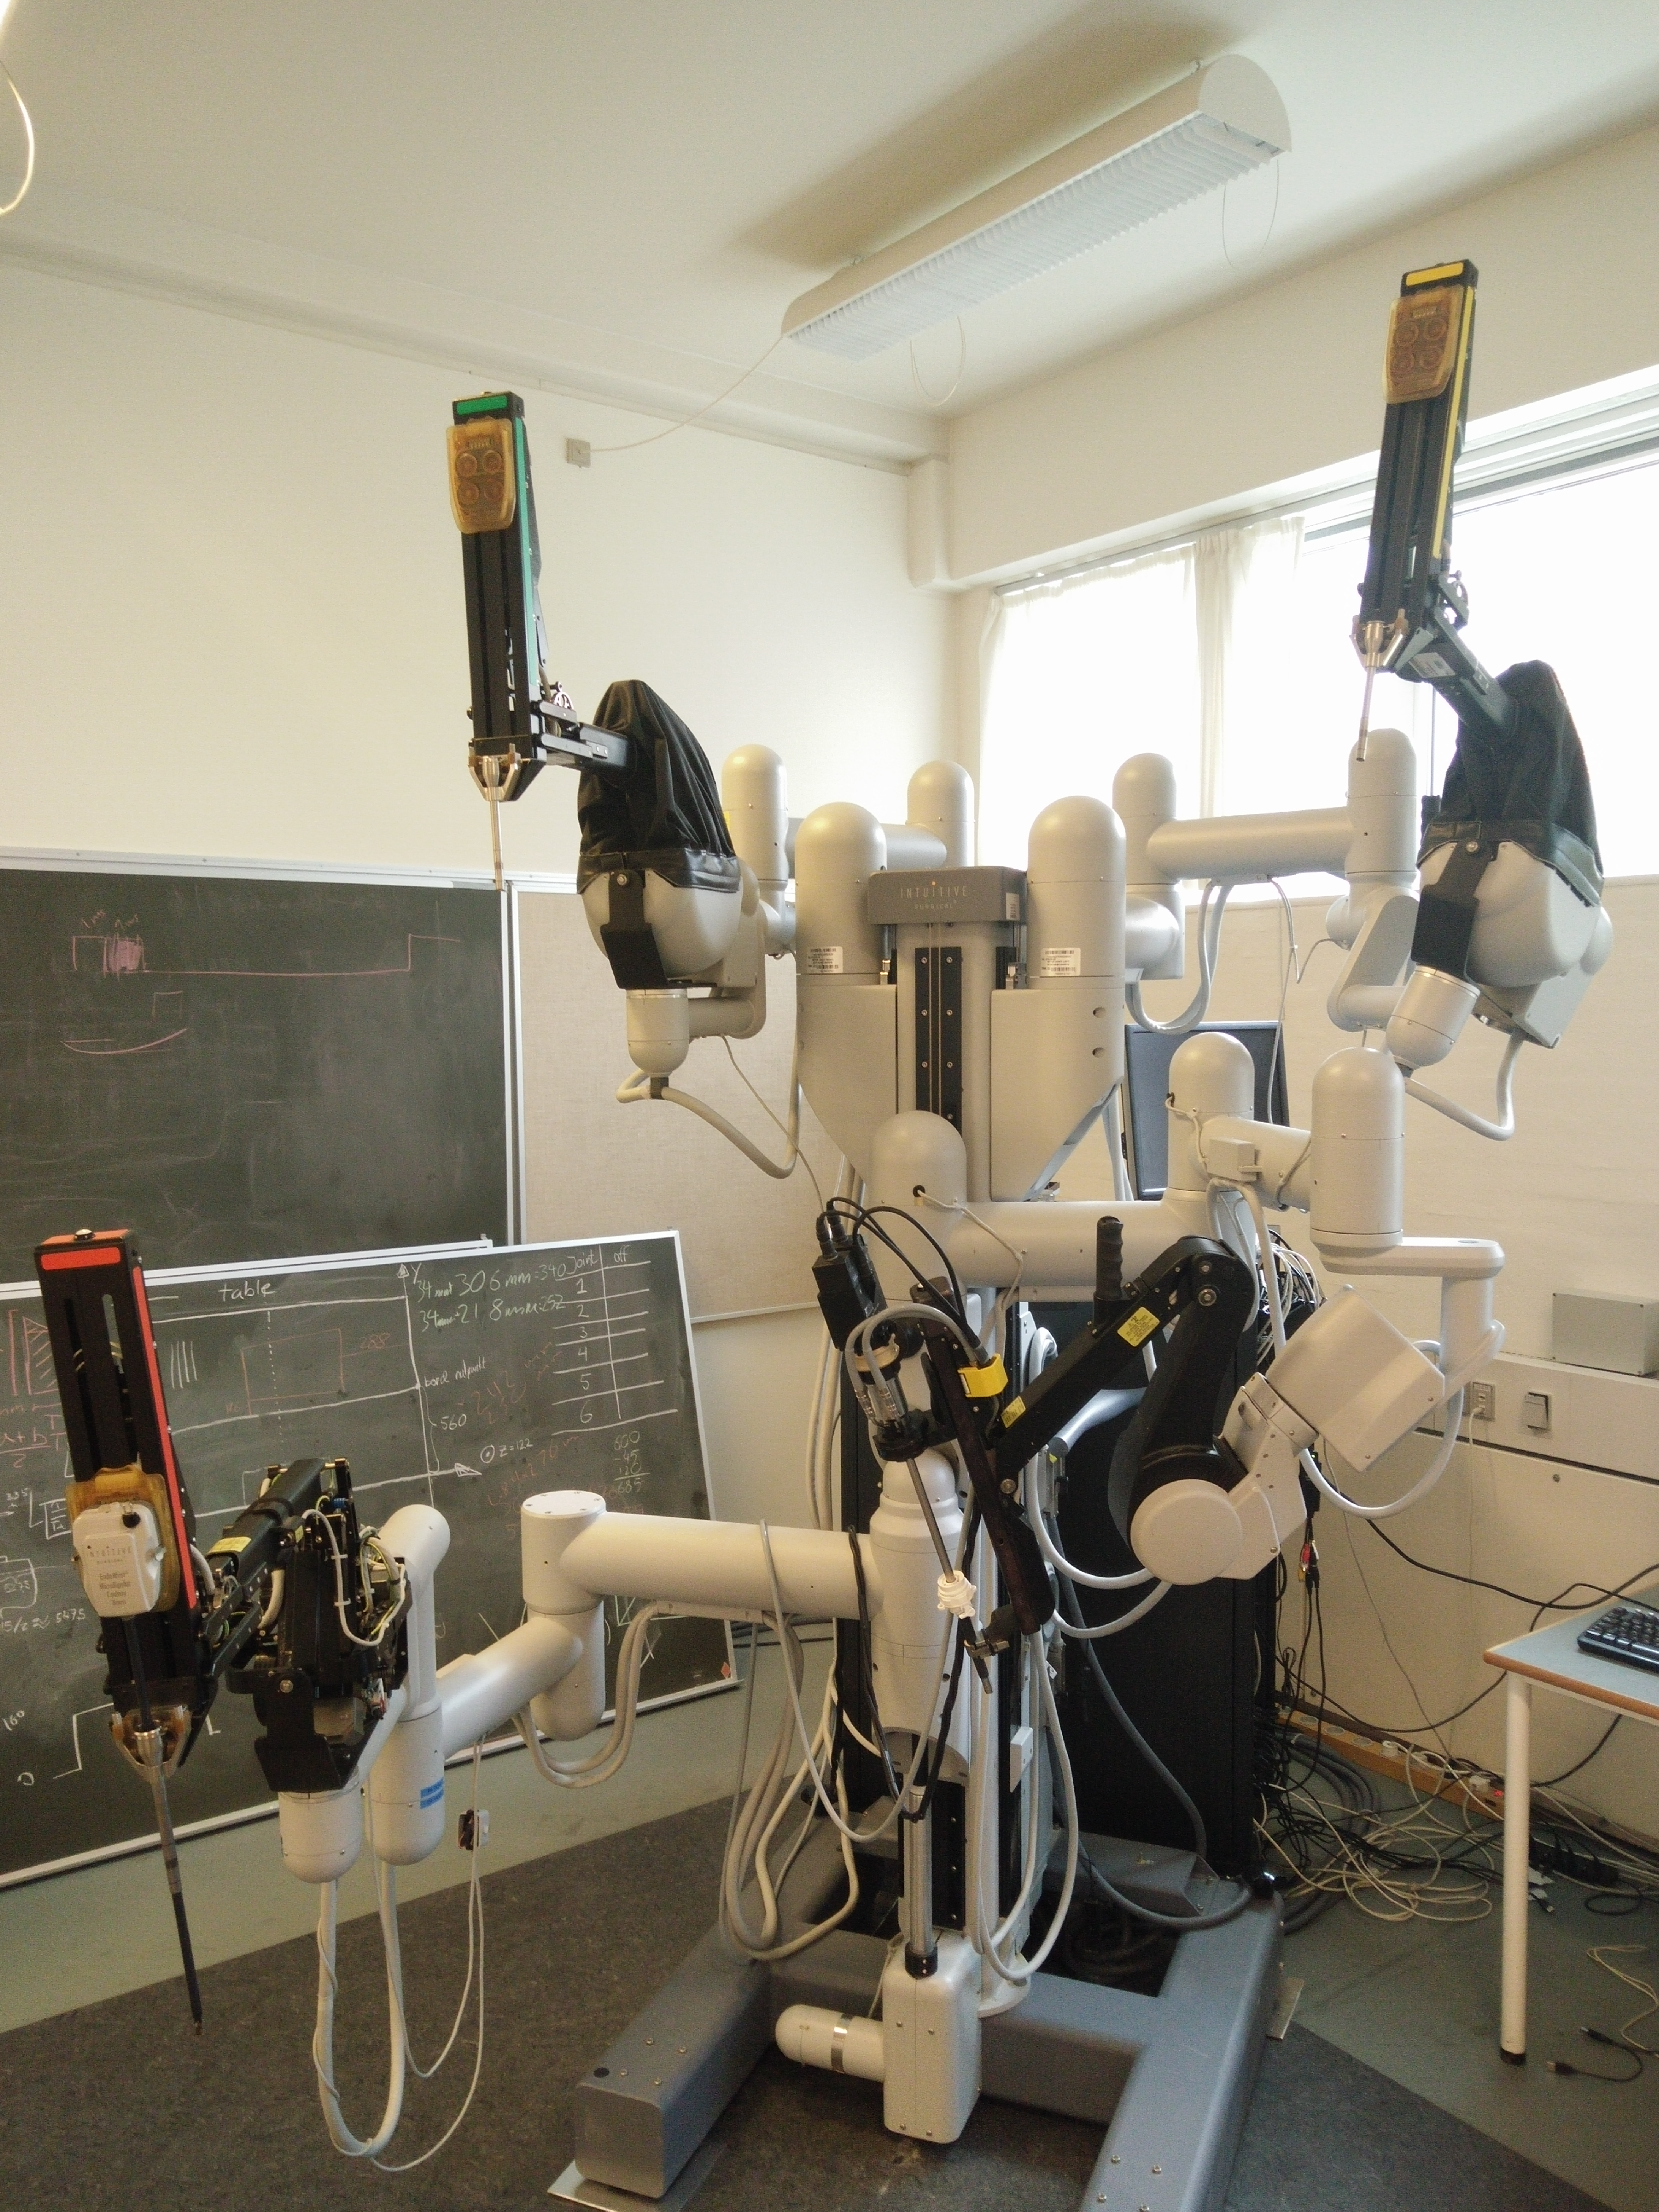
\includegraphics[width=\linewidth]{DavinciRobot.jpg}
		\caption{The da Vinci robot or slave manipulator.}
		\label{fig:davincirobot}
	\end{subfigure}
	\begin{subfigure}{.45\textwidth}
		\centering
		\vspace{12pt}
		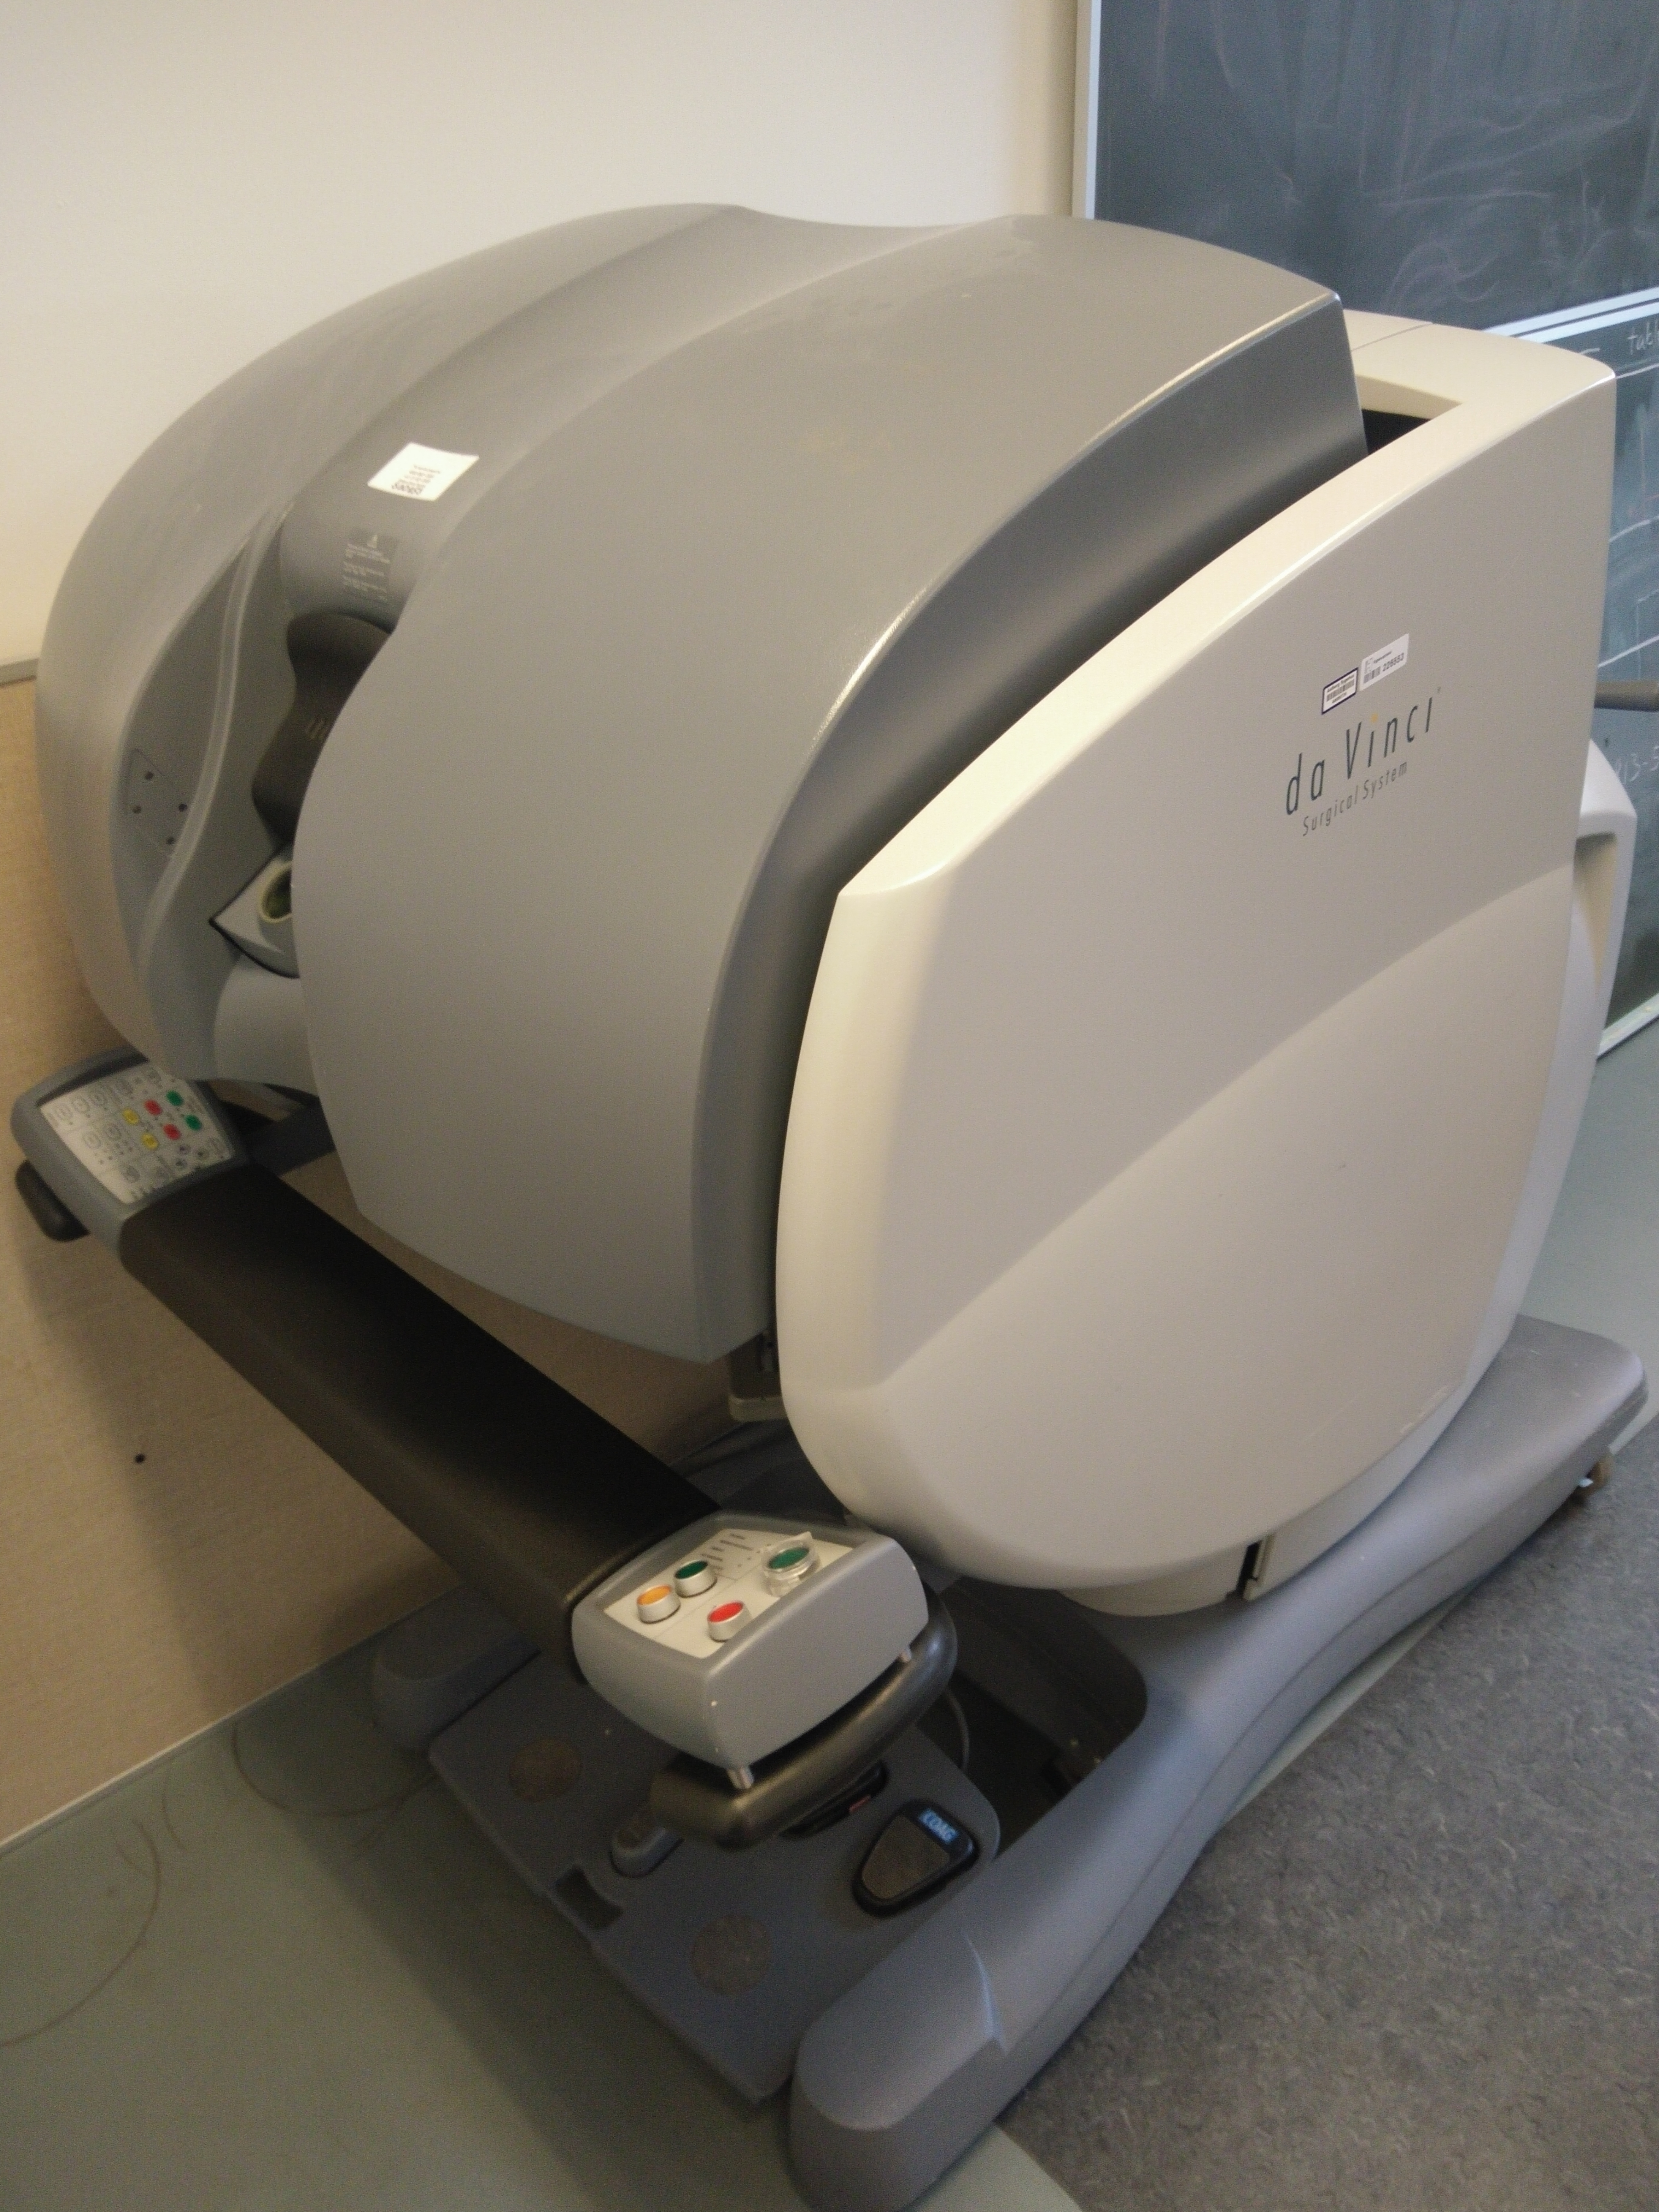
\includegraphics[width=\linewidth]{masterconsole.jpg}
		\caption{The master console for controlling the slave manipulator.}
		\label{fig:mastermani}
	\end{subfigure}
\caption{Full view of the da Vinci surgery system which include the slave manipulator and the master console}
\label{fig:fulldavinci}
\end{figure}

It consists of two main parts, a master console, see \figref{fig:mastermani}, and a slave manipulator, see \figref{fig:davincirobot}.

\begin{itemize}
\item The surgeon uses the master console to control the slave manipulator. It consists of two eye pieces, which display a high resolution 3D view of the surgery for the surgeon. 
\item The slave manipulator is the robot which is controlled from the master console by the surgeon. It consists of four arms that with 6-7 actuated \gls{DOF} each, depending on the tool attached.
\end{itemize}


%a replacement master controller called a Geo magic touch is implemented, see \secref{sec:geo_magic}.


\subsection*{Slave manipulator arm}
The slave manipulator arm consists of three parts, arm, hand and tool, see \figref{fig:davinciarmrobot}.

\begin{figure}[H]
	\centering
		\centering
		\includegraphics[width=0.85\linewidth]{davincirobotarm_label.jpg}
		\caption{One extended arm of the da Vinci robot. The tool (EndoWrist), hand and arm are marked.}
		\label{fig:davinciarmrobot}
\end{figure}


\begin{enumerate}
\item Arm:

The arm of the da Vinci is the part being the furthest away from the patient. 
During surgery, it is locked to a specific position. Between surgeries, its 6 \gls{DOF}s can be adjusted.
\item Hand

The hand is at the end of the arm and has three \gls{DOF}, two rotational and one translational, which can be actuated during surgery. 
\item End-effector tool (EndoWrist)

The end-effector tool is connected to the hand, it is only capable of doing rotational movement on its own. Together the tool and the hand have 6 - 7 movable \gls{DOF} that can be actuated. The tool is the instrument which interacts with the patient during surgery. There are several different tools available, each with their own functionality. 
\end{enumerate}

The present project concentrates on implementing haptic feedback control for the end-effector called EndoWrist. Controlling the robot arm is not a subject of this project. The end-effector was separated from the da Vinci system.
The da Vinci's master console controller lacks actuation. In order to be able to provide haptic feedback, a Geomagic Touch, see \secref{sec:geo_magic}, has been implemented as a replacement. The original master console will not be further analyzed. 